\documentclass[
  bibliography=totoc,     % Literatur im Inhaltsverzeichnis
  captions=tableheading,  % Tabellenüberschriften
  parskip=half,	% Abstand als Absatz
  %titlepage=firstiscover, % Titelseite ist Deckblatt
]{scrartcl}

% LaTeX2e korrigieren.
\usepackage{fixltx2e}
% Warnung, falls nochmal kompiliert werden muss
\usepackage[aux]{rerunfilecheck}

% Zeichnet Grpahen aus matplotlib
\usepackage{pgf}

% deutsche Spracheinstellungen
\usepackage{polyglossia}
\setmainlanguage{german}

% unverzichtbare Mathe-Befehle
\usepackage{amsmath}
% viele Mathe-Symbole
\usepackage{amssymb}
% Erweiterungen für amsmath
\usepackage{mathtools}

% Fonteinstellungen
\usepackage{fontspec}
\defaultfontfeatures{Ligatures=TeX}

\usepackage[
  math-style=ISO,    % \
  bold-style=ISO,    % |
  sans-style=italic, % | ISO-Standard folgen
  nabla=upright,     % |
  partial=upright,   % /
]{unicode-math}

\setmathfont{Latin Modern Math}
\setmathfont[range={\mathscr, \mathbfscr}]{XITS Math}
\setmathfont[range=\coloneq]{XITS Math}
\setmathfont[range=\propto]{XITS Math}
% make bar horizontal, use \hslash for slashed h
\let\hbar\relax
\DeclareMathSymbol{\hbar}{\mathord}{AMSb}{"7E}
\DeclareMathSymbol{ℏ}{\mathord}{AMSb}{"7E}

% richtige Anführungszeichen
\usepackage[autostyle]{csquotes}

% Zahlen und Einheiten
\usepackage[
  locale=DE,                   % deutsche Einstellungen
  separate-uncertainty=true,   % Immer Fehler mit \pm
  per-mode=symbol-or-fraction, % m/s im Text, sonst Brüche
]{siunitx}

% chemische Formeln
\usepackage[version=3]{mhchem}

% schöne Brüche im Text
\usepackage{xfrac}

% Floats innerhalb einer Section halten
\usepackage[section, below]{placeins}
% Captions schöner machen.
\usepackage[
  labelfont=bf,        % Tabelle x: Abbildung y: ist jetzt fett
  font=small,          % Schrift etwas kleiner als Dokument
  width=0.9\textwidth, % maximale Breite einer Caption schmaler
]{caption}
% subfigure, subtable, subref
\usepackage{subcaption}

% Grafiken können eingebunden werden
\usepackage{graphicx}
% größere Variation von Dateinamen möglich
\usepackage{grffile}

% Standardplatzierung für Floats einstellen
\usepackage{float}
\floatplacement{figure}{htbp}
\floatplacement{table}{htbp}

% schöne Tabellen
\usepackage{booktabs}

% Seite drehen für breite Tabellen
\usepackage{pdflscape}

% Position der Seitenzahl
\usepackage{geometry}
\geometry{a4paper, left=2.5cm, right=2cm, top=3cm, bottom=4cm} 

% Größe der Plots
\newcommand{\pltwidth}{13cm}

% Literaturverzeichnis
\usepackage{biblatex}
% Quellendatenbank
\addbibresource{lit.bib}

% Hyperlinks im Dokument
\usepackage[
  unicode,
  pdfusetitle,    % Titel, Autoren und Datum als PDF-Attribute
  pdfcreator={},  % PDF-Attribute säubern
  pdfproducer={}, % "
]{hyperref}
% erweiterte Bookmarks im PDF
\usepackage{bookmark}

% Trennung von Wörtern mit Strichen
\usepackage[shortcuts]{extdash}

\author{
  Vincent Latko
  \texorpdfstring{
    \\
    \href{mailto:vincent.latko@tu-dortmund.de}{vincent.latko@tu-dortmund.de}
  }{}%
  \texorpdfstring{\and}{, }
  Marian Kleineberg
  \texorpdfstring{
    \\
    \href{mailto:marian.kleineberg@tu-dortmund.de}{marian.kleineberg@tu-dortmund.de}
  }{}
}
\publishers{TU Dortmund – Fakultät Physik}


%%% Hier definiert man Titel, Autor und Datum %%%%%%%%%%%%%%%%%%%%%%%%%%%%%%%%%

\subject{Versuchsprotokoll}
\title{Rastertunnelmikroskop}
\date{
  Durchführung: 18.04.2016
  \hspace{3em}
  Abgabe: 21.04.2016
}

%%%%%%%%%%%%%%%%%%%%%%%%%%%%%%%%%%%%%%%%%%%%%%%%%%%%%%%%%%%%%%%%%%%%%%%%%%%%%%%

\begin{document}

\maketitle
\thispagestyle{empty}
%\tableofcontents
%\newpage

\section{Einleitung}
Dieser Versuch behandelt die Funktion der Rastertunnelmikroskopie. Der Name leitet sich daraus ab, dass Festkörperproben mit einer Spitze abgerastert werden und daraus Bilder der Oberfläche der jeweiligen Festkörper aufgenommen werden können.

\noindent Im Folgenden wird der theoretische Hintergrund der STM (scanning tunneling microscopy) erläutert und die Messung für Proben HOPG (highly oriented pyrolytic graphite) und Gold ausgewertet.
\section{Theorie}
\subsection{Theorie des Lichts}
Ein Laser emittiert hoch intensives monochromatisches Licht, also Licht einer einzigen Wellenlänge beziehungsweise Farbe. Das bedeutet auch, dass das Licht möglichst kohärent ist, also der Kontrast der Interferenzmuster maximiert wird. In der Realität ist das Licht nicht perfekt monochromatisch, da im Lasergehäuse die Neonatome nicht still stehen, sondern eine eigene Geschwindigkeit haben und somit der Doppler-Effekt bezüglich des emittierten Lichts eintritt. Somit ist auch die perfekte Kohärenz nicht möglich.

\noindent Licht wird im Teilchenbild durch Emission von Photonen beim Übergang eines Elektrons von einem Niveau eines Atoms in ein energetisch günstigeres beschrieben. Es existieren zwei Arten der Emission. Die stimulierte und spontane Emission. Die spontane Emission entsteht durch Fluktuationen in der Ladungsverteilung der Atome. Die stimulierte Emission ist die für den Laser relevante, da dabei im Gegensatz zum statistischen Ereignis der spontanen Emission, die Abstrahlung von Photonen kontrolliert werden kann. Dabei werden zwei Photonen emittiert, von denen eines die selbe Energie, Phase und Ausbreitungsrichtung wie das stimulierende beziehungsweise einfallende Photon hat.

\noindent Darüber hinaus gibt es noch die Absorption. Hierbei wird ein auf das Atom treffende Photon, welches die Energie des Überganges hat, absorbiert indem ein Elektron ein Energieniveau aufsteigt.

\noindent Ein zwar nicht für die Funktion eines Lasers ausreichendes, aber grundlegendes System ist das Zwei-Niveau-System. Dabei wird die Besetzungsdichte \(n_2\) des angeregten Zustandes durch die Absorption erhöht und durch die spontane und stimulierte Emission verringert. Um hochintensive Licht zu erzeugen, sollte bei einem Laser die stimulierte Emission der Absorbtion überwiegen, sodass das \(n_2>n_1\) ist, wobei \(n_1\) die Besetzungsdichte im Grundzustand bedeutet.

\subsection{Theorie des Lasers}
Ein Laser besteht im wesentlichen aus drei Komponenten. Eine ist das aktive Lasermedium. Dabei handelt es sich um ein Gas, einen Festkörper oder eine Flüssigkeit. Bei dem Laser dieses Versuchs wird ein Gas verwendet. Die notwendige Bedingung an ein Lasermedium stellt die Fähigkeit zur Besetzungsinversion dar, also \(n_2>n_1\). Als Lasermedium dient hier Neon.

\noindent Eine weitere Komponente ist die Pumpquelle. Durch das so genannte Pumpen, wird dem Lasermedium Energie zugeführt und somit Zustände höherer Energie häufiger besetzt, als diejenigen niedrieger. Es wird also eine Besetzungsinversion erzeugt. Entscheidend dafür, ob ein Niveau durch pumpen angeregt werden kann, ist die Temperatur des Systems, also die Besetzung der Niveaus bezüglich der Boltzmann-Verteilung, die Anregungsrate sowie die Lebensdauer der Zustände im angeregten Zustand. Die Energie wird an das Neon durch Stöße zweiter Art übergeben. Diese sind Stöße zweier Atome, von denen eines im Angeregten und das andere im Grundzustand ist. Bei einem Stoß zweiter Art besteht dann eine Wahrscheinlichkeit, das angeregte Atom in den Grundzustand und das im Grundzustand verweilende in den angeregten Zustand zu bringen. Die Pumpquelle ist hier Helium. Das Verhältnis von Helium zu Neon ist bei diesem Laser fünf zu eins.

\noindent Die dritte Komponente ist der Resonator. Er besteht aus einem möglichst vollständig reflektierenden und einem teildurchlässigen Spiegel sowie einem Laserrohr, in dem sich das Lasermedium befindet und das an den Enden in Brewsterfenster mündet. Die Brewsterfenster sind 

%BREWSTERFENSTER ERKLÄREN

. Diese stehen in einem Abstand \(L\)  voneinander auf der optischen Achse und haben die Krümmungsradien \(r_1\) und \(r_2\). Dadurch entsteht eine optische Rückkopplung, bei der das Licht mehrmals das Lasermedium durchläuft und ein selbsterregender Oszillator entsteht. 

\begin{figure}
	\centering
	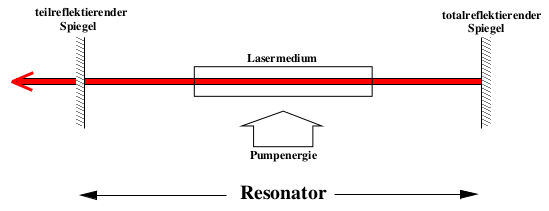
\includegraphics[width=0.5\textwidth]{resonator}
	\caption{Laser-Resonator}
	\label{fig:resonator}
\end{figure}

\noindent Die Abbildung \ref{fig:resonator} zeigt einen grober Aufbau eines Resonators.

\noindent Durch den Resonator legt der Laserstrahl einen möglichst langen Weg im Lasermedium zurück und wird somit verstärkt. Die Stabilität ist daher vom Resonatortyp und der Form der Spiegel abhängig. Optimal sind für einen Laser konfokale Spiegel, da diese einen in einem Punkt zusammenfallenden Brennpunkt gewährleisten und somit geringe Verluste bezüglich der Resonatorspiegel aufweisen.

\noindent Eine Stabilitätsbedingung für den Resonator ist gegeben durch:

\begin{equation}
0\le g_1\cdot g_2<1
\end{equation}

\noindent Dabei sind die \(g_i\) durch \(g_i=1-\frac{L}{r_i}\) gegeben.

\noindent Es existiert eine Mehrzahl von Frequenzen, die die Resonanzbedingung erfüllen. Diese sind über \(f=\frac{nc}{\pi L}\) gegeben. Es gibt sowohl transversale als auch longitudinale Moden. Erste entstehen, durch Unebenheiten der Spiegel oder Verkippungen. Die Moden werden als \(\text{TEM}_{lpq}\) (transverse electromagnetic mode) bezeichnet, dabei sind \(l\) und \(p\) die Knoten in x- und y-Richtung und heißen transversale Modenzahl. Die Verluste steigen mit der Modenzahl, sodass nur wenige Moden isoliert werden können. Die Mode mit höchster Symmetrie und mit den wenigsten Verlusten ist die \(\text{TEM}_00\) Grundmode.
\section{Versuch}
\subsection{Versuchsaufbau}
Die benutzten Werkzeuge sind der PtIr-Draht, ein Seitenschneider, eine Zange, eine Pinzette, die Proben HOPG und Gold, sowie das Rastertunnelmikroskop mit einer Abdichtung in der eine Lupe mit zehnfacher Verstärkung verbaut ist.

\noindent Die in Kapitel \ref{kap2} beschriebene Schwierigkeit der Vibrationen wird durch einen Schwingungsdämpfenden Tisch der zusätzlich auf vier dämpfenden Füßen steht, gelöst. Der Tisch ist aus Granit um eine möglichst schwere Grundfläche zu gewährleisten. Die Füße sind aus Gummi, um ein Verrutschen der Vorrichtung zu verhindern und sind intern mit Federn ausgestattet um die letzten Schwingungen zu dämpfen. Auf dem Tisch ist die Messvorrichtung installiert.

\noindent Ein Aufbau ist in Abbildung \ref{fig:Aufbau1} \cite{handbuch} dargestellt. 

\begin{figure}
	\centering
		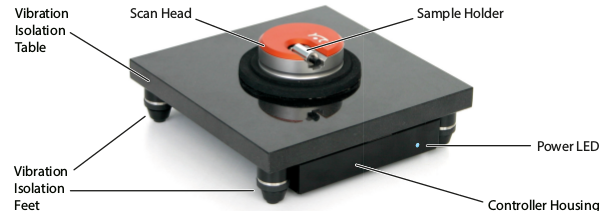
\includegraphics[width=0.5\textwidth]{Aufbau1.png}
	\caption{Rastertunnelmikroskop}
	\label{fig:Aufbau1}
\end{figure}

\noindent Ein genauerer Einblick in die Messvorrichtung wird in Abbildung \ref{fig:Aufbau2} gegeben.

\begin{figure}
	\centering
		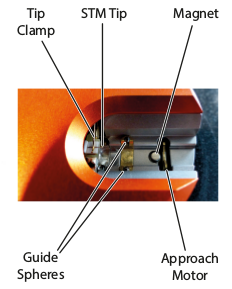
\includegraphics[width=0.5\textwidth]{Aufbau2.png}
	\caption{Messvorrichtung}
	\label{fig:Aufbau2}
\end{figure}

\noindent Durch den Magnet wird die Probenhalterung, die an ihrer Spitze selbst magnetisiert ist um die Probe, die auf einer kreisförmigen Metallscheibe liegt, an ihrem Ort fixiert. Die Spitze wird unter einen Bügel in eine dafür vorgesehene Furche gelegt und dort festgehalten. Die Probe kann auf metall Kugeln durch den Motor an den gewünschten Ort verschoben werden.

\subsection{Versuchsdurchführung}
Zunächst wurden die Werkzeuge mit 2-Propanol gereinigt. Mit der Zange wurde ein Stück des Drahts festgehalten und mit dem Seitenschneider wurde dann (nahezu parallel zur Zange gehalten) eine Spitze aus dem Draht gerissen. Zuletzt wurde die Spitze auf die richtige Größe geschnitten und mit der Pinzette unter den Bügel gelegt.

\noindent Daraufhin wurde eine Probe in die Messvorrichtung gelegt. Sie kann über die thermisch isolierte Halterung mit der Hand angefasst transportiert werden. Die Abdichtung wurde darauf gestellt.

\noindent Der Rest der Durchführung geschah mit dem Programm ''Nanosurf NaioSTM''.

\noindent Als Erstes wurde über den ''more''-Button das Menü für die SPM-Parameter geöffnet und unter ''Imaging'' -> ''Imaging Modes'' -> ''Scan Mode'', ''Scan Fw. \& Bw.'' ausgewählt.

\noindent Mit ''Advance'' bzw. ''Approach'' konnte die Spitze an die Probe gefahren werden. Nachdem die richtigen Parameter unter ''Parameters'' eingestellt wurden, musste noch eine Spannung (\(50\)mV) zwischen Spitze und Probe angelegt werden. Dies geschah durch die Einstellung unter ''Mode Properties''.
\section{Auswertung}
\subsection{Isobare Molwärme}
Um die Molwärme bei konstantem Druck aus den gegebenen Messwerten zu bestimmen, muss zunächst die Zeitdifferenz für alle gemessenen Zeiten errechnet werden. Aus dieser kann dann die elektrische Energie mit der Formel \ref{ELEKTRISCHEENERGIE} berechnet werden. Die Temperatur aus dem Widerstand mit Hilfe der Formel \ref{TEMPERATUR} bestimmt.

\noincent Mit diesen Werten kann nun die spezifische Wärme berechnet werden. Die Molwärme ergibt sich dann aus Formel \ref{MOLWÄRME}.

\noindent Die benutzten Messwerte sind Tabelle \ref{fig:tab1} zu entnehmen.   

\begin{table}[H]
	\begin{center}
		\begin{tabular}{c c c c c c}
			\toprule
			\(t\)/s & \(R\)/\(\Omega\) & \(I\)/mA & \(U\)/V & \(T\)/K & \(\sigma_T\)/K\\
			\midrule
			0		&22,2		&133,9	&14,14	&81,76	&0,24 \\
			300		&25,2		&136,0	&14,24	&88,84	&0,24 \\
			600		&27,6		&146,1	&15,32	&94,52	&0,24 \\
			900		&30,0		&160,0	&16,79	&100,22	&0,24 \\
			1200	&33,1		&166,4	&17,48	&107,60	&0,24 \\
			1500	&36,2		&175,7	&18,49	&115,00	&0,24 \\
			1800	&39,2		&180,3	&18,98	&122,19	&0,24 \\
			2100	&44,9		&180,8	&18,98	&135,92	&0,24 \\
			2400	&48,8		&180,0	&18,98	&145,37	&0,24 \\
			2700	&52,7		&180,3	&18,98	&154,85	&0,24 \\
			3000	&56,3		&180,4	&18,98	&163,64	&0,24 \\
			3300	&59,8		&180,5	&18,98	&172,22	&0,25 \\
			3600	&63,3		&180,6	&18,98	&180,84	&0,25 \\
			3900	&66,6		&180,7	&18,98	&188,99	&0,25 \\
			4260	&70,4		&180,8	&18,98	&198,41	&0,25 \\
			4620	&73,3		&180,9	&18,98	&205,63	&0,25 \\
			4980	&77,8		&181,0	&18,98	&216,87	&0,25 \\
			5340	&81,0		&181,0	&18,98	&224,89	&0,25 \\
			5760	&85,6		&181,1	&18,98	&236,48	&0,25 \\
			6120	&89,0		&181,1	&18,98	&245,09	&0,25 \\
			6480	&92,5		&181,2	&18,98	&253,98	&0,25 \\
			6840	&96,1		&181,2	&18,98	&263,15	&0,26 \\
			7200	&99,7		&181,3	&18,98	&272,36	&0,26 \\
			7560	&102,5		&181,3	&18,98	&279,55	&0,26 \\
			7980	&106,6		&181,3	&18,98	&290,11	&0,26 \\
			8400	&110,2		&181,3	&18,98	&299,42	&0,26 \\
			\bottomrule
		\end{tabular}
		\caption{Messdaten und Temperatur}
		\label{fig:tab1}
	\end{center}
\end{table}

\noindent Hierbei wird für die Zeit ein Reaktionsfehler von \(\sigma_t=1\text{s}\), für den Widerstand ein Ablesefehler von \(\sigma_\Omega=0,1\text{Ohm}\) und für Strom und Spannung jeweils ein Ablesefehler von \(\sigma_I=0,01\text{mA}\) und \(\sigma_U=0,01\text{V}\) angenommen.

\noindent Da in der Molwärme und Energie Differenzen auftreten, wird der letzte Messwert nicht mehr in die Berechnung eingehen.

\noindent Die Messunsicherheit der Energie berechnet sich aus der Formel für die Gauß'sche Fehlerfortpflanzung:

\begin{equation}
\sigma_E=\sqrt{(I\Delta t\cdot\sigma_U)^2 + (U\Delta t\cdot\sigma_I)^2 + (UI\cdot\sigma_t)^2}
\end{equation}

\noindent Die Messunsicherheit für die Molwärme errechnet sich zu:

\begin{equation}
\sigma_{C_p}=\sqrt{\left(\frac mM\cdot\frac{1}{\Delta t}\cdot\sigma_E\right)^2+\left(-\frac mM\cdot\frac{E}{\Delta t^2}\cdot\sigma_t\right)^2 }
\end{equation}

\noindent Die Ergebnisse für die Molwärme und Energie sind Tabelle \ref{fig:tab2} zu entnehmen.

\begin{table}[H]
	\begin{center}
		\begin{tabular}{c c c c c c}
			\toprule
			\(E\)/J & \(\sigma_E\)/J & \(\Delta t\)/s & \(\Delta T\)/K & \(C_p\)/\(\frac{\text{J mol}}{\text{K}}\) & \(\sigma_{C_p}\)/							\(\frac{\text{J mol}}{\text{K}}\) \\
			\midrule
			568,00	&2,68	&300	&81,76	&14,91	&0,71\\
			580,99	&2,74	&300	&88,84	&19,00	&1,12\\
			671,48	&3,17	&300	&94,52	&21,91	&1,30\\
			805,92	&3,79	&300	&100,22	&20,29	&0,93\\
			872,60	&4,11	&300	&107,59	&21,89	&1,00\\
			974,61	&4,59	&300	&115,00	&25,18	&1,19\\
			1026,62	&4,84	&300	&122,19	&13,89	&0,35\\
			1029,48	&4,85	&300	&135,92	&20,26	&0,74\\                           
			1024,92	&4,83	&300	&145,37	&20,08	&0,86\\
			1026,63	&4,84	&300	&154,85	&21,69	&0,86\\ 
			1027,20	&4,84	&300	&163,64	&22,24	&0,90\\
			1027,76	&4.85	&300	&172,22	&22,17	&0,90\\
			1028,34	&4,85	&300	&180,84	&23,44	&1,01\\
			1234,69	&4,85	&360	&188,99	&24,35	&0,91\\
			1235,37	&4,85	&360	&198,41	&31,81	&1,56\\
			1236,05	&4.86	&360	&205,63	&20,43	&0,65\\
			1236,74	&4.86	&360	&216,87	&28,63	&1,27\\                
			1442,86	&4.86	&360	&224,89	&23,14	&0,76\\                  
			1237,42	&4.86	&360	&236,40	&26,73	&1,12\\                    
			1237,42	&4.86	&360	&245,09	&25,87	&1,05\\
			1238,10	&4.86	&360	&253,98	&25,07	&0,98\\ 
			1238,10	&4.86	&360	&263,15	&24,97	&0,99\\            
			1238,78	&4.86	&360	&272,36	&32,02	&1,62\\
			1445,25	&4.86	&420	&279,55	&25,43	&0,88\\
			1445,25	&4.86	&420	&290,11	&28,84	&1,14\\
			\bottomrule
		\end{tabular}
		\caption{Werte für die zugeführte Energie und die davon errechnete Molwärme}
		\label{fig:tab2}
	\end{center}
\end{table}

\subsection{Isochore Molwärme}
Die Molwärme bei konstantem Volumen wird über die Korrekturformel \ref{KORREKTURFORMEL} berechnet. Hierzu ist das Wissen über die Werte des Ausdehnungskoeffizienten von Relevanz. In Abbildung \ref{fig:tab3} sind Werte für \(\alpha\) für bestimmte Temperaturen angegeben.

\begin{table}[H]
	\begin{center}
		\begin{tabular}{c c}
			\toprule
			\(T\)/K & \(\alpha/\text{K}\cdot10^{-6}\)\\
			\midrule
			70	&7,00\\
			80	&8,50\\
			90	&9,75\\
			100	&10,70\\
			110	&11,50\\
			120	&12,10\\
			130	&12,65\\
			140	&13,15\\
			150	&13,60\\
			160	&13,90\\
			170	&14,25\\
			180	&14,50\\
			190	&14,75\\
			200	&14,95\\
			210	&15,20\\
			220	&15,40\\
			230	&15,60\\
			240	&15,75\\
			250	&15,90\\
			260	&16,10\\
			270	&16,25\\
			280	&16,35\\
			290	&16,50\\
			300	&16,65\\
			\bottomrule
		\end{tabular}
		\caption{Linearer Ausdehnungskoeffizient \(\alpha\) von Kupfer in Abhängigkeit von der Temperatur}
		\label{fig:tab3}
	\end{center}
\end{table}

\noindent Um Werte für die gegebenen Temperaturen aus Tabelle \ref{fig:tab1} zu bekommen, werden die Werte aus Tabelle \ref{fig:tab3} als Stützstellen mit Hilfe eines Polynoms sechsten Grades interpoliert:

\begin{equation*}
p(x)=ax^6+bx^5+cx^4+dx^3+ex^2+fx+g\quad.
\end{equation*}

\begin{figure}
	\centering
		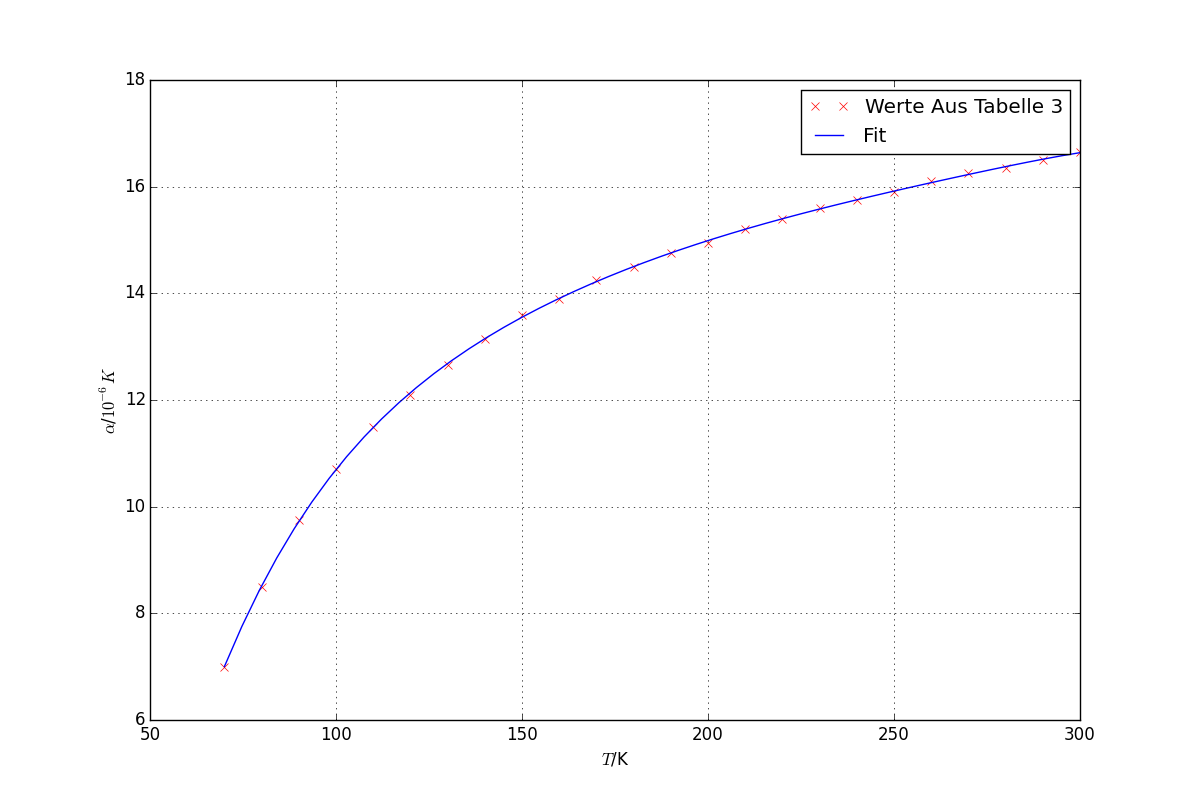
\includegraphics[width=0.5\textwidth]{inter.png}
	\caption{Interpolation des Polynoms}
	\label{fig:abb1}
\end{figure}

\noindent Für die Korrekturformel wird noch der Kompressionsmodul und das Molvolumen benötigt. Hierfür werden Literaturwerten verwendet: \(\kappa=1,378\cdot10^{11}\frac{\text{N}}{\text{m}^2}\), \(V_0=7,11\cdot10^{-6}\frac{\text{m}^3}{\text{mol}}\). 

\noindent Die Werte für die Molwärme und die passenden Ausdehnungskoeffizienten sind der Tabelle \ref{fig:tab4} zu entnehmen.

\begin{table}[H]
	\begin{center}
		\begin{tabular}{c c c c c}
			\toprule
			\(T\)/K & \(\alpha/\text{K}\cdot10^{-6}\) & \(\sigma_\alpha/\text{K}\cdot10^{-5}\) & \(C_V\)/\(\frac{\text{J mol}}{\text{K}}\) & \(\sigma_{C_V}\)\(\frac{\text{J mol}}{\text{K}}\) \\
			\midrule
			81,76&	8,75		&1,38	&14,85	&0,72\\
			88,84&	9,59		&1,63	&18,93	&1,14\\
			94,52&	10,18	&1,85	&21,82	&1,33\\
			100,22&	10,71	&2,11	&20,19	&1,01\\
			107,60&	13,10	&2,48	&21,77	&1,13\\
			115,00&	11,82	&2,90	&25,04	&1,38\\
			122,19&	12,27	&3,37	&13,73	&0,95\\
			135,92&	12,97	&4,44	&20,05	&1,56\\
			145,37&	13,37	&5,34	&19,85	&1,97\\
			154,85&	13,73	&6,38	&21,44	&2,54\\
			163,64&	14,02	&7,49	&21,96	&3,16\\
			172,22&	14,29	&8,73	&21,86	&3,89\\
			180,84&	14,52	&10,15	&23,10	&4,80\\
			188,99&	14,73	&11,65	&23,98	&5,79\\
			198,41&	14,95	&13,63	&31,41	&7,30\\
			205,63&	15,11	&15,32	&20,01	&8,42\\
			216,87&	15,34	&18,32	&28,17	&10,82\\
			224,89&	15,49	&20,74	&22,66	&12,76\\
			236,48&	15,69	&24,71	&26,21	&16,21\\
			245,09&	15,84	&28,04	&25,33	&19,22\\
			253,98&	15,98	&31,89	&24,50	&22,84\\
			263,15&	16,12	&36,30	&24,37	&27,18\\
			272,36&	16,26	&41,23	&31,39	&32,25\\
			279,55&	16,37	&45,46	&24,76	&36,70\\
			290,11&	16,51	&52,33	&28,14	&44,23\\
			\bottomrule
		\end{tabular}
		\caption{Ausdehnungskoeffizient für gemessene Temperaturen und Molwärme bei konstantem Volumen}
		\label{fig:tab4}
	\end{center}
\end{table}

\noindent Die Messunsicherheit \(\sigma_\alpha\) ergibt sich aus:

\begin{equation}
\sigma_\alpha=\sqrt{((6aT^5+5bT^4+4cT^3+3ddT^2+2eT+f)\sigma_T)^2+(T^5\cdot\sigma_a)^2+(T^4\cdot\sigma_b)^2+(T^3\cdot\sigma_c)^2+(T^2\cdot\sigma_d)^2+(T\cdot\sigma_e)^2+(\sigma_f)^2+(0\cdot\sigma_g)^2}
\end{equation}

\noindent Die Messunsicherheit für die isochore Molwärme ergibt sich aus:

\begin{equation}
\sigma_{C_V}=\sqrt{(\Delta\sigma_{C_p})^2 + (9\alpha^2\kappa V_0\cdot\sigma_T)^2 + (18\alpha\kappa V_0T\cdot\sigma_\alpha)^2}
\end{equation}

\noindent Die Molwärme bei konstantem Volumen gegen die Temperatur im linearen Diagramm wird in Abbildung \ref{fig:abb2} dargestellt.

\begin{figure}
	\centering
		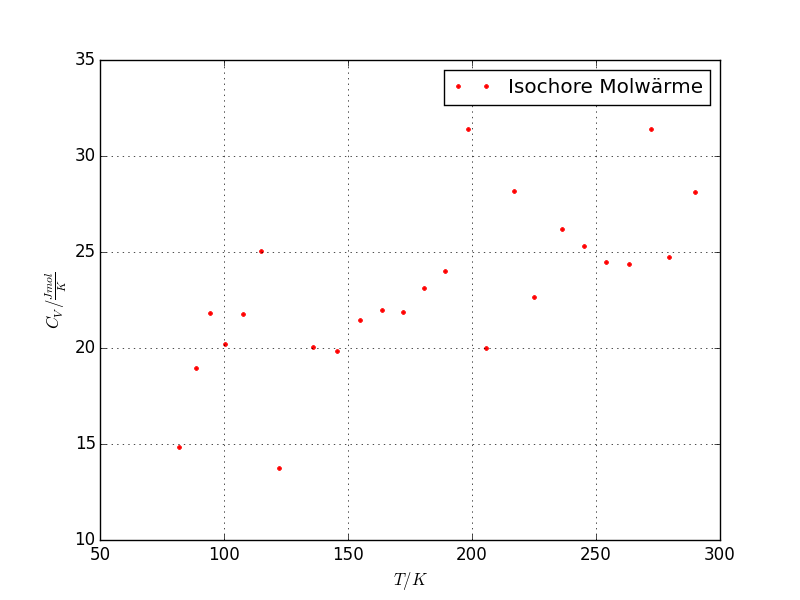
\includegraphics[width=0.5\textwidth]{cv.png}
	\caption{Isochore Molwärme und Grenzwert}
	\label{fig:abb2}
\end{figure}

\subsection{Debye-Temperatur}
Die Werte für\(\frac{\theta_\text{D}}{T}\) werden aus Tabelle \ref{tab4} bestimmt. Dabei sind die Zahlen der ersten Spalte die Nachkommastellen. Die Debye-Temperatur wird dann durch Multiplikation mit der Temperatur berechnet. Das Ergebnis ist Tabelle \ref{fig:tab5} zu entnehmen.

\begin{figure}
	\centering
		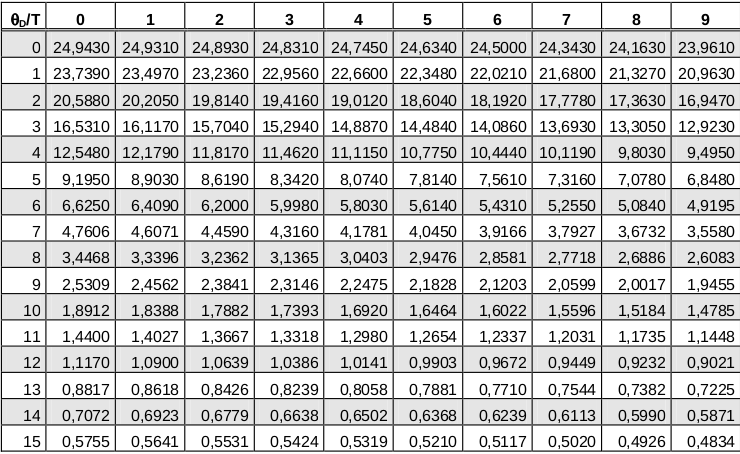
\includegraphics[width=0.5\textwidth]{debye.png}
	\caption{Debye-Temperatur für bestimmte Molwärme}
	\label{fig:abb3}
\end{figure}

\begin{table}[H]
	\begin{center}
		\begin{tabular}{c c c c}
			\toprule
			\(T\)/K & \(C_V\)/\(\frac{\text{J mol}}{\text{K}}\) & \(\frac{\theta_\text{D}}{T}\) & \(\theta_D\)/K \\
			\midrule
			81,76	&14,85	&4,3		&351,57\\
			88,84	&18,93	&4,2		&373,13\\
			94,52	&21,82	&7,1		&671,09\\
			100,22	&20,19	&1,2		&120,26\\
			107,60	&21,77	&7,1		&763,96\\
			115,00	&25,04	&0,0		&0,00\\
			122,19	&13,73	&7,3		&891,99\\
			135,93	&20,05	&2,2		&299,02\\
			145,37	&19,85	&2,2		&319,81\\
			154,85	&21,44	&8,1		&1254,29\\
			163,64	&21,96	&6,1		&998,20\\
			\bottomrule
		\end{tabular}
		\caption{Ergebnisse für die Debye-Temperatur}
		\label{fig:tab5}
	\end{center}
\end{table}

\noindent Der Wert \(C_V\) ist offensichtlich ein Messfehler, weswegen er nicht in die Berechnung des Mittelwerts eingeht.

\noindent Der Mittelwert dieser Werte für die Debye-Temperatur lautet dann:

\begin{equation}
\frac{1}{10}\sum\limits_{i=1}^{10}{\theta_{\text{D}}}_i=\overline{\theta_\text{D}}=549,39
\end{equation}

\noindent Die Standardabweichung ist dann:

\begin{equation}
\sigma_\theta=\sqrt{\frac{1}{9}\sum\limits_{i=1}^{10}({\theta_{\text{D}}}_i-\overline \theta_{\text{D}})^2}=118,63
\end{equation}

\subsection{Debye-Frequenz}
Zur Berechnung der theoretischen Debye-Frequenz wird die Forderung \ref{FORDERUNG} betrachtet. Aus dieser folgt der Ausdruck \ref{OMEGADEBYE}, mit dem es möglich ist, die Debye-Frequenz analytisch zu bestimmen.

\noindent Die noch zu bestimmenden Größen sind die Anzahl der Freiheitsgrade \(N_L\) und das Volumen der Probe \(L\).

\begin{equation*}
N_L=\frac{m}{m_\text{Atom}}=\frac{0,342\text{kg}}{63,55\cdot 1,66\cdot10^{-27}\text{kg}}=3,24\cdot10^{24}
\end{equation*}

\begin{equation*}
L^3=\frac{m}{\rho_\text{Kupfer}}=\frac{0,342\text{kg}}{8,92\cdot10^3\frac{kg}{\text{m}^3}}=3,83\cdot10^{-5}\text{m}^3
\end{equation*}

\noindent Dabei ist \(m_\text{Atom}\) die Masse eines einzelnen Kupferatoms. Für die Geschwindigkeiten wird \(v_\text{long}=4,7\cdot10^3\frac{\text{m}}{\text{s}}\) und \(v_\text{trans}=2,26\cdot10^3\frac{\text{m}}{\text{s}}\) verwendet.

\noindent Daraus ergibt sich für die Debye-Frequenz:

\begin{equation*}
\omega_\text{D}=5,38\cdot10^{13}\frac{1}{\text{s}}
\end{equation*}

\noindent Daraus lässt sich auch die theoretische Debye-Temperatur berechnen. Mit der Formel \ref{THETADEBYE} lautet die theoretische Temperatur:

\begin{equation*}
\theta_\text{D}=411,22\text{K}\quad.
\end{equation*}
\section{Diskussion}

Die Messung des Gittervektors von Graphit mithilfe der Rastertunnelmikroskopie erfolgte relativ genau.
Der Literaturwert liegt im Fehlerbereich des gemessenen Wertes.
Der gemessene Wert weicht um $8,1\%$ vom Literaturwert ab.

Bei der Messung mit Gold enthalten die Aufnahmen starkes Rauschen.
Abgesehen vom Rauschen ergeben sich weitere Artefakte am Rand der Aufnahme, die größer sind als die eigentlichen Stufenkanten.
Diese könnten durch eine gekrümmte Probenoberfläche oder durch Fehler im Rastertunnelmikroskop erklärt werden.

Die Höhe der Stufenkante im aufgenommenen Profil stimmt mit dem Literaturwert überein.

Die Qualität der Messungen mit dem verwendeten Rastertunnelmikroskop hängt von einer Reihe von Faktoren ab, die unterschiedlich gut kontrolliert werden können.
Beispielsweise können Verunreinigungen des Aufbaus oder eine schlechte Messspitze das Ergebnis verschlechtern.
Ein weiterer Faktor, der verbessert werden könnte, ist die Einstellung der PID-Regler.

\printbibliography

\end{document}
